% answers.tex —— 2005 年·全国卷Ⅱ·文科 · 参考答案与详细解析片段
% 由 tools/generate_projects.py 依来源总账自 2005/2005_数学真题_全国2文_试题.md + 2005/2005_数学真题_全国2文_解析正文.md + 2005/2005_数学真题_全国2文_答案要点.md 生成，勿手改（改源 MD 后重跑）


\begin{gktip}
固定源 PDF 为印刷页码 250–251 的两页题面，不附答案。以下解析均依据固定源独立复算；第 20 题图形在 LaTeX 工程中以 TikZ/PGFPlots 矢量源重绘。
\end{gktip}

\begin{answer}
\gksolhead{1}{}

\textbf{题目}：

函数 $f(x)=|\sin x+\cos x|$ 的最小正周期是\mbox{（　　）}

（A）$\dfrac{\pi}{4}$\quad（B）$\dfrac{\pi}{2}$\quad（C）$\pi$\quad（D）$2\pi$

\Needspace{4\baselineskip}
\textbf{解析}

\nopagebreak[4]
\[
|\sin x+\cos x|=\sqrt2\left|\sin\left(x+\frac\pi4\right)\right|,
\]

故最小正周期为 $\pi$。

\gkanswer{答案：C}

\end{answer}
\begin{answer}
\gksolhead{2}{}

\textbf{题目}：

正方体 $ABCD-A_1B_1C_1D_1$ 中，$P\text{、}Q\text{、}R$ 分别是 $AB\text{、}AD\text{、}B_1C_1$ 的中点。那么，正方体的过 $P\text{、}Q\text{、}R$ 的截面图形是\mbox{（　　）}

（A）三角形\quad（B）四边形\quad（C）五边形\quad（D）六边形

\Needspace{4\baselineskip}
\textbf{解析}

与单位正方体建立坐标，过三个中点的截面平面为 $x+y-z=1/2$，在立方体内依次切出六个顶点，故截面为六边形。

\gkanswer{答案：D}

\end{answer}
\begin{answer}
\gksolhead{3}{}

\textbf{题目}：

函数 $y=x^2-1\ (x\leqslant0)$ 的反函数是\mbox{（　　）}

（A）$y=\sqrt{x+1}\ (x\geqslant-1)$\quad（B）$y=-\sqrt{x+1}\ (x\geqslant-1)$

（C）$y=\sqrt{x+1}\ (x\geqslant0)$\quad（D）$y=-\sqrt{x+1}\ (x\geqslant0)$

\Needspace{4\baselineskip}
\textbf{解析}

\Needspace{5\baselineskip}
由 $y=x^2-1$ 且 $x\leqslant0$，反解得 $x=-\sqrt{y+1}$，交换变量后反函数为

\nopagebreak[4]
\[
y=-\sqrt{x+1},\quad x\geqslant-1\text{。}
\]

\gkanswer{答案：B}

\end{answer}
\begin{answer}
\gksolhead{4}{}

\textbf{题目}：

已知函数 $y=\tan\omega x$ 在 $\left(-\dfrac{\pi}{2},\dfrac{\pi}{2}\right)$ 内是减函数，则\mbox{（　　）}

（A）$0<\omega\leqslant1$\quad（B）$-1\leqslant\omega<0$\quad（C）$\omega\geqslant1$\quad（D）$\omega\leqslant-1$

\Needspace{4\baselineskip}
\textbf{解析}

在给定区间中 $\sec^2(\omega x)>0$，减函数要求 $\omega<0$；为了没有额外间断点还需 $|\omega|\leqslant1$，故 $-1\leqslant\omega<0$。

\gkanswer{答案：B}

\end{answer}
\begin{answer}
\gksolhead{5}{}

\textbf{题目}：

抛物线 $x^2=4y$ 上一点 $A$ 的纵坐标为 $4$，则点 $A$ 与抛物线焦点的距离为\mbox{（　　）}

（A）$2$\quad（B）$3$\quad（C）$4$\quad（D）$5$

\Needspace{4\baselineskip}
\textbf{解析}

抛物线焦点为 $(0,1)$，点 $A$ 的横坐标为 $\pm4$，故焦点距离为 $\sqrt{4^2+3^2}=5$。

\gkanswer{答案：D}

\end{answer}
\begin{answer}
\gksolhead{6}{}

\textbf{题目}：

双曲线 $\dfrac{x^2}{4}-\dfrac{y^2}{9}=1$ 的渐近线方程是\mbox{（　　）}

（A）$y=\pm\dfrac23x$\quad（B）$y=\pm\dfrac49x$\quad（C）$y=\pm\dfrac32x$\quad（D）$y=\pm\sqrt3x$

\Needspace{4\baselineskip}
\textbf{解析}

\Needspace{5\baselineskip}
由 $\dfrac{x^2}{4}-\dfrac{y^2}{9}=0$ 得渐近线

\nopagebreak[4]
\[
y=\pm\frac32x\text{。}
\]

\gkanswer{答案：C}

\end{answer}
\begin{answer}
\gksolhead{7}{}

\textbf{题目}：

如果数列 $\{a_n\}$ 是等差数列，则\mbox{（　　）}

（A）$a_1+a_8<a_4+a_5$\quad（B）$a_1+a_8=a_4+a_5$\quad（C）$a_1+a_8>a_4+a_5$\quad（D）$a_1a_8=a_4a_5$

\Needspace{4\baselineskip}
\textbf{解析}

等差数列中 $a_1+a_8=a_4+a_5$。

\gkanswer{答案：B}

\end{answer}
\begin{answer}
\gksolhead{8}{}

\textbf{题目}：

$(x-\sqrt2y)^{10}$ 的展开式中 $x^6y^4$ 项的系数是\mbox{（　　）}

（A）$840$\quad（B）$-840$\quad（C）$210$\quad（D）$-210$

\Needspace{4\baselineskip}
\textbf{解析}

\Needspace{5\baselineskip}
取四个 $-\sqrt2y$ 因子，系数为

\nopagebreak[4]
\[
\binom{10}{4}(-\sqrt2)^4=210\cdot4=840\text{。}
\]

\gkanswer{答案：A}

\end{answer}
\begin{answer}
\gksolhead{9}{}

\textbf{题目}：

已知点 $A(\sqrt3,1)$、$B(0,0)$、$C(\sqrt3,0)$。设 $\angle BAC$ 的平分线 $AE$ 与 $BC$ 相交于 $E$，那么有 $\overrightarrow{BC}=\lambda\overrightarrow{CE}$，其中 $\lambda$ 等于\mbox{（　　）}

（A）$2$\quad（B）$\dfrac12$\quad（C）$-3$\quad（D）$-\dfrac13$

\Needspace{4\baselineskip}
\textbf{解析}

角平分线定理给出 $BE:EC=AB:AC=2:1$，所以 $\overrightarrow{BC}=-3\overrightarrow{CE}$。

\gkanswer{答案：C}

\end{answer}
\begin{answer}
\gksolhead{10}{}

\textbf{题目}：

已知集合 $M=\{x\mid x^2-3x-28\leqslant0\}$，$N=\{x\mid x^2-x-6>0\}$，则 $M\cap N$ 为\mbox{（　　）}

（A）$\{x\mid-4\leqslant x<-2\text{ \text{或} }3<x\leqslant7\}$\quad（B）$\{x\mid-4<x\leqslant-2\text{ \text{或} }3\leqslant x<7\}$

（C）$\{x\mid x\leqslant-2\text{ \text{或} }x>3\}$\quad（D）$\{x\mid x<-2\text{ \text{或} }x\geqslant3\}$

\Needspace{4\baselineskip}
\textbf{解析}

\nopagebreak[4]
\[
M=[-4,7],\qquad N=(-\infty,-2)\cup(3,+\infty),
\]

故 $M\cap N=[-4,-2)\cup(3,7]$。

\gkanswer{答案：A}

\end{answer}
\begin{answer}
\gksolhead{11}{}

\textbf{题目}：

点 $P$ 在平面上作匀速直线运动，速度向量 $\vec v=(4,-3)$（即点 $P$ 的运动方向与 $\vec v$ 相同，且每秒移动的距离为 $|\vec v|$ 个单位）。设开始时点 $P$ 的坐标为 $(-10,10)$，则 $5$ 秒后点 $P$ 的坐标为\mbox{（　　）}

（A）$(-2,4)$\quad（B）$(-30,25)$\quad（C）$(10,-5)$\quad（D）$(5,-10)$

\Needspace{4\baselineskip}
\textbf{解析}

五秒位移为 $(20,-15)$，所以点的坐标为 $(10,-5)$。

\gkanswer{答案：C}

\end{answer}
\begin{answer}
\gksolhead{12}{}

\textbf{题目}：

$\triangle ABC$ 的顶点 $B$ 在平面 $\alpha$ 内，$A\text{、}C$ 在 $\alpha$ 的同一侧，$AB\text{、}BC$ 与 $\alpha$ 所成的角分别是 $30^\circ$ 和 $45^\circ$。若 $AB=3$，$BC=4\sqrt2$，$AC=5$，则 $AC$ 与 $\alpha$ 所成的角为\mbox{（　　）}

（A）$60^\circ$\quad（B）$45^\circ$\quad（C）$30^\circ$\quad（D）$15^\circ$

\Needspace{4\baselineskip}
\textbf{解析}

\Needspace{5\baselineskip}
两条边相对平面的竖直分量为 $3/2$、$4$，差为 $5/2$。因 $AC=5$，线面角 $\theta$ 满足

\nopagebreak[4]
\[
\sin\theta=\frac{5/2}{5}=\frac12,
\]

故 $\theta=30^\circ$。

\gkanswer{答案：C}

\end{answer}
\begin{answer}
\gksolhead{13}{}

\textbf{题目}：

在 $\dfrac83$ 和 $\dfrac{27}{2}$ 之间插入三个数，使这五个数成等比数列，则插入的三个数的乘积为\gkblank{}。

\Needspace{4\baselineskip}
\textbf{解析}

设公比 $q$，由端项关系得 $q=3/2$，插入数为 $4,6,9$，乘积 $216$。

\gkanswer{答案：216}

\end{answer}
\begin{answer}
\gksolhead{14}{}

\textbf{题目}：

圆心为 $(1,2)$ 且与直线 $5x-12y-7=0$ 相切的圆的方程为\gkblank{}。

\Needspace{4\baselineskip}
\textbf{解析}

圆心到直线距离为 $2$，故方程为 $(x-1)^2+(y-2)^2=4$。

\gkanswer{答案：$(x-1)^2+(y-2)^2=4$}

\end{answer}
\begin{answer}
\gksolhead{15}{}

\textbf{题目}：

在由数字 $0,1,2,3,4,5$ 所组成的没有重复数字的四位数中，不能被 $5$ 整除的数共有\gkblank{}个。

\Needspace{4\baselineskip}
\textbf{解析}

四位数总数 $300$，能被 $5$ 整除的有末位 $0$ 的 $60$ 个和末位 $5$ 的 $48$ 个，故不能被 $5$ 整除的有 $192$ 个。

\gkanswer{答案：192}

\end{answer}
\begin{answer}
\gksolhead{16}{}

\textbf{题目}：

下面是关于三棱锥的四个命题：

① 底面是等边三角形，侧面与底面所成的二面角都相等的三棱锥是正三棱锥；

② 底面是等边三角形，侧面都是等腰三角形的三棱锥是正三棱锥；

③ 底面是等边三角形，侧面的面积都相等的三棱锥是正三棱锥；

④ 侧棱与底面所成的角都相等，且侧面与底面所成的二面角都相等的三棱锥是正三棱锥。

其中，真命题的编号是\gkblank{}。（写出所有真命题的编号）

\Needspace{4\baselineskip}
\textbf{解析}

① 侧面二面角相等使顶点在底面内的投影到三边距离相等，成立；② 仅要求三个侧面为等腰三角形时可构造非正三棱锥，故不成立；③ 等面积只保证到三边所在直线的距离相等，投影可为外心或外心型位置，故不成立；④ 侧棱与底面角相等使投影到三个顶点等距，再结合二面角条件得到正三棱锥。真命题为 ①④。

\gkanswer{答案：①④}

\end{answer}
\begin{answer}
\gksolhead{17}{}

\textbf{题目}：

已知 $\alpha$ 为第二象限的角，$\sin\alpha=\dfrac35$，$\beta$ 为第一象限的角，$\cos\beta=\dfrac5{13}$，求 $\tan(2\alpha-\beta)$ 的值。

\Needspace{4\baselineskip}
\textbf{解析}

\Needspace{5\baselineskip}
由 $\sin\alpha=3/5$ 且 $\alpha$ 为第二象限角，$\cos\alpha=-4/5$；由 $\cos\beta=5/13$ 且 $\beta$ 为第一象限角，$\sin\beta=12/13$。计算正切差角公式：

\nopagebreak[4]
\[
\tan2\alpha=-\frac{24}{7},
\qquad
\tan(2\alpha-\beta)
=\frac{-24/7-12/5}{1-288/35}
=\frac{204}{253}\text{。}
\]

\gkanswer{答案：$\dfrac{204}{253}$}

\end{answer}
\begin{answer}
\gksolhead{18}{}

\textbf{题目}：

甲、乙两队进行一场排球比赛。根据以往经验，单局比赛甲队胜乙队的概率为 $0.6$，本场比赛采用五局三胜制，即先胜三局的队获胜，比赛结束，设各局比赛相互间没有影响，求：

（1） 前三局比赛甲队领先的概率；

（2） 本场比赛乙队以 $3:2$ 取胜的概率。（精确到 $0.001$）

\Needspace{4\baselineskip}
\textbf{解析}

\gksubpart{(1)}

\Needspace{5\baselineskip}
前三局甲领先为至少胜两局：

\nopagebreak[4]
\[
\binom32(0.6)^2(0.4)+(0.6)^3=0.648\text{。}
\]

\gksubpart{(2)}

\Needspace{5\baselineskip}
乙队以 $3:2$ 获胜需前四局各胜两局且第五局乙胜，概率

\nopagebreak[4]
\[
\binom42(0.6)^2(0.4)^2(0.4)=0.13824\approx0.138\text{。}
\]

\gkanswer{答案（1）：$0.648$}

\gkanswer{答案（2）：$0.138$}

\end{answer}
\begin{answer}
\gksolhead{19}{}

\textbf{题目}：

\Needspace{5\baselineskip}
已知 $\{a_n\}$ 是各项均为正数的等差数列，$\lg a_1\text{、}\lg a_2\text{、}\lg a_4$ 成等差数列。又

\nopagebreak[4]
\[
b_n=\frac1{a_{2^n}},\qquad n=1,2,3,\ldots\text{。}
\]

（1） 证明 $\{b_n\}$ 为等比数列；

（2） 如果数列 $\{b_n\}$ 前 $3$ 项的和等于 $\dfrac7{24}$，求数列 $\{a_n\}$ 的首项 $a_1$ 和公差 $d$。

\Needspace{4\baselineskip}
\textbf{解析}

\gksubpart{(1)}

\Needspace{5\baselineskip}
设 $a_1=x$、公差为 $d$。对数成等差给出

\nopagebreak[4]
\[
(x+d)^2=x(x+3d)\Longrightarrow d(d-x)=0\text{。}
\]

\gksubpart{(2)}

\Needspace{5\baselineskip}
若 $d=0$，前三项 $b_n=1/x$ 的和为 $7/24$，得 $x=72/7$。若 $d=x$，则 $a_n=nx$，$b_n=1/(2^nx)$，由

\nopagebreak[4]
\[
\frac1{2x}+\frac1{4x}+\frac1{8x}=\frac7{24}
\]

得 $x=3$。所以两组解为 $(72/7,0)$ 与 $(3,3)$。

\gkanswer{答案（1）：$\{b_n\}$ 为等比数列}

\gkanswer{答案（2）：$(a_1,d)=\left(\dfrac{72}{7},0\right)$ 或 $(a_1,d)=(3,3)$}

\end{answer}
\begin{answer}
\gksolhead{20}{}

\textbf{题目}：

如图，四棱锥 $P-ABCD$ 中，底面 $ABCD$ 为矩形，$PD\perp$ 底面 $ABCD$，$AD=PD$，$E\text{、}F$ 分别为 $CD\text{、}PB$ 的中点。
\nopagebreak[4]
\begin{center}% 2005 年全国卷Ⅱ文科第 20 题：直棱锥
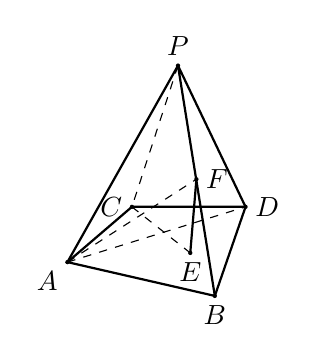
\begin{tikzpicture}[>=stealth,scale=0.78]
  \coordinate (A) at (0,0); \coordinate (B) at (2.4,-0.55);
  \coordinate (C) at (1.05,0.9); \coordinate (D) at (2.9,0.9);
  \coordinate (P) at (1.8,3.2); \coordinate (E) at (2.0,0.15);
  \coordinate (F) at (2.1,1.35);
  \draw[thick] (A)--(B)--(D)--(C)--cycle;
  \draw[thick] (P)--(A) (P)--(B) (P)--(D);
  \draw[dashed] (P)--(C) (A)--(D) (C)--(D);
  \draw[thick] (E)--(F);
  \draw[dashed] (A)--(F) (C)--(E);
  \fill (P) circle (1pt) node[above] {$P$};
  \fill (A) circle (1pt) node[below left] {$A$};
  \fill (B) circle (1pt) node[below] {$B$};
  \fill (C) circle (1pt) node[left] {$C$};
  \fill (D) circle (1pt) node[right] {$D$};
  \fill (E) circle (1pt) node[below] {$E$};
  \fill (F) circle (1pt) node[right] {$F$};
\end{tikzpicture}
\end{center}
\nopagebreak[4]
（1） 求证：$EF\perp$ 平面 $PAB$；

（2） 设 $AB=\sqrt2BC$，求 $AC$ 与平面 $AEF$ 所成的角的大小。

\Needspace{4\baselineskip}
\textbf{解析}

\gksubpart{(1)}

\Needspace{5\baselineskip}
取 $BC=b$，则可设

\nopagebreak[4]
\[
A=(0,0,0),\ B=(\sqrt2b,0,0),\ D=(0,b,0),\ C=(\sqrt2b,b,0),\ P=(0,b,b)\text{。}
\]

中点 $E\text{、}F$ 如题，得到 $\overrightarrow{EF}$ 同时垂直于 $AB\text{、}AP$，故 $EF\perp$ 平面 $PAB$。

\gksubpart{(2)}

\Needspace{5\baselineskip}
平面 $AEF$ 的法向量与 $\overrightarrow{AC}$ 作线面角计算，得到

\nopagebreak[4]
\[
\sin\theta=\frac{\sqrt3}{6}\text{。}
\]

\gkanswer{答案（1）：$EF\perp$ 平面 $PAB$}

\gkanswer{答案（2）：所成锐角 $\theta$ 满足 $\sin\theta=\dfrac{\sqrt3}{6}$}

\end{answer}
\begin{answer}
\gksolhead{21}{}

\textbf{题目}：

设 $a$ 为实数，函数 $f(x)=x^3-x^2-x+a$。

（1） 求 $f(x)$ 的极值；

（2） 当 $a$ 在什么范围内取值时，曲线 $y=f(x)$ 与 $x$ 轴仅有一个交点。

\Needspace{4\baselineskip}
\textbf{解析}

\gksubpart{(1)}

\nopagebreak[4]
\[
f'(x)=3x^2-2x-1=(3x+1)(x-1)\text{。}
\]

\gksubpart{(2)}

\Needspace{5\baselineskip}
故极大值为 $a+5/27$，极小值为 $a-1$。要使三次曲线只有一个与 $x$ 轴的交点，需两个极值严格同侧：

\nopagebreak[4]
\[
a+\frac5{27}<0\quad\text{\text{或}}\quad a-1>0,
\]

即 $a<-5/27$ 或 $a>1$。

\gkanswer{答案（1）：极大值为 $a+\dfrac5{27}$，在 $x=-\dfrac13$ 时取得；极小值为 $a-1$，在 $x=1$ 时取得}

\gkanswer{答案（2）：$a<-\dfrac5{27}$ 或 $a>1$}

\end{answer}
\begin{answer}
\gksolhead{22}{}

\textbf{题目}：

$P\text{、}Q\text{、}M\text{、}N$ 四点都在椭圆 $x^2+\dfrac{y^2}{2}=1$ 上，$F$ 为椭圆在 $y$ 轴正半轴上的焦点。已知 $\overrightarrow{PF}$ 与 $\overrightarrow{FQ}$ 共线，$\overrightarrow{MF}$ 与 $\overrightarrow{FN}$ 共线，且 $\overrightarrow{PF}\cdot\overrightarrow{MF}=0$。求四边形 $PMQN$ 的面积的最小值和最大值。

\Needspace{4\baselineskip}
\textbf{解析}

\Needspace{5\baselineskip}
椭圆焦点为 $(0,1)$。过焦点、方向角为 $\theta$ 的弦长为

\nopagebreak[4]
\[
L(\theta)=\frac{2\sqrt2}{1+\cos^2\theta}\text{。}
\]

\Needspace{5\baselineskip}
题设两弦垂直，四边形的对角线为两弦，故

\nopagebreak[4]
\[
S=\frac8{(1+\cos^2\theta)(1+\sin^2\theta)}\text{。}
\]

令 $u=\cos^2\theta$，分母 $2+u-u^2$ 取值区间为 $[2,9/4]$，所以面积最小值为 $16/9$，最大值为 $2$。

\gkanswer{答案：面积最小值为 $\dfrac{16}{9}$，最大值为 $2$}

\end{answer}